% Todo:

\documentclass[12pt]{article}
\usepackage{xeCJK}
\usepackage{fontspec}
%\setCJKmainfont{SimSun}
\setCJKmainfont[BoldFont=SimHei,ItalicFont=KaiTi]{SimSun}
\setCJKsansfont{SimHei}
% \setCJKmonofont{SimKai}
% \setmainfont{Arial}

\usepackage{cite}
\usepackage{graphicx}
\usepackage{float}
\usepackage{amsfonts}
% \usepackage{amsmath}	% for \tag
\usepackage{amssymb}	% for \multimap
% \usepackage{stmaryrd}
\usepackage{color}
%\usepackage[square,numbers]{natbib}
%\nocopyright
%\usepackage{latexsym,amsmath,amssymb,graphicx,hyperref}
%\usepackage{times} % gives you a bit more space if needed
\usepackage{titlesec}		% change color of section headings
\usepackage{verbatim} % for block comments

\titleformat{\section}
{\color{blue}\normalfont\Large\bfseries}
{\color{blue}\thesection}{1em}{}
\renewcommand\abstractname{\textcolor{blue}{Abstract}}

\newcommand{\concept}[1]{\textbf{\textcolor{blue}{#1}}}
% \definecolor{LogicColor}{rgb}{0.4,0.1,0.4}  % Magenta
\definecolor{grey}{rgb}{0.5,0.5,0.5}
\definecolor{LogicColor}{rgb}{0.4,0.1,0.4}  % Magenta

\newcommand{\english}[1]{\rmfamily \textit{``#1''}\rmfamily}
\newcommand{\formula}[1]{\ttfamily\textcolor{LogicColor}{#1}\rmfamily}

\newcommand{\df}{f} %probability density function
\newcommand{\dfo}{f1} %other probability density function
\newcommand{\fv}{x} %fuzzy variable
\newcommand{\tab}{\hspace*{1cm}}
\newcommand{\zand}{\; \tilde{\wedge} \;}
\newcommand{\zor}{\; \tilde{\vee} \;}
\newcommand{\PimpL}{\leftarrowtriangle}
\newcommand{\com}{\multimap}
\newcommand{\comL}{\circ \hspace{-0.4em} - \,}
\newcommand{\mul}{}
\newcommand{\loves}{loves }
\newcommand{\heart}{\, \heartsuit \,}

\setlength{\oddsidemargin}{1cm}
\setlength{\evensidemargin}{1cm}
\setlength{\textwidth}{14cm}

\title{\textcolor{blue}{Genifer 3.0 white paper}}
\author{YKY (\textit{甄景贤})}
% \institute{}

\begin{document}

\tab\tab\tab \parbox{11cm}{\textit{I am an enthusiast, but not a crank in the sense that I have some pet theories as to the proper construction of a flying machine. I wish to avail myself of all that is already known and then, if possible, add my mite to help on the future worker who will attain final success.}}
\vspace{-0.5cm}
\begin{flushright}
\textemdash Wilbur Wright
\end{flushright}

\sffamily

{\let\newpage\relax\maketitle}

\maketitle
\setlength{\parindent}{0em}
\setlength{\parskip}{1.5ex plus0.5ex minus1.2ex}

\begin{abstract}
\noindent Introduces the Genifer3 logic engine.
\end{abstract}

\section{Background}

Genifer3 is ``neo-classical'', logic-based AI similar to OpenCog and NARS.  Genifer4 attempts to transition logic to a vector space setting and employ continuous iterative methods, but its details have not been worked out yet.

\concept{Propositional logic} concerns with propositions (``sentences'') which can be assigned \textit{truth values} and which have no \textit{internal structure}.  For example the formula $P \wedge Q$.  Propositional logic is isomorphic to Boolean algebra.  Its proof problem is called SAT (\concept{satisfiability}) and is famously NP-complete.  \concept{Resolution} is a proof algorithm for propositional logic.

\concept{Predicate logic} gives formulas internal structure via predicates such as \formula{loves(john, mary)}.  Predicate logic allows to have patterns such as \formula{loves(X, Y)} where X and Y are variables.  Logic rules containing patterns are matched to facts via the \concept{unification} algorithm;  This is known as \textit{pattern-matching}.  For example, this rule defines ``grandfather'':\\
\tab\formula{grandfather(X,Z) $\leftarrow$ father(X,Y) $\wedge$ father(Y,Z)}\\

The proof procedure for predicate logic combines \textbf{unification} with \textbf{resolution}.  This procedure is undecidable in the worst case \textemdash \, it follows because first-order logic is Turing universal and the \textit{halting problem} dictates that such a proof procedure must be undecidable.

Genifer3 is different from classical logic in the following ways:
\begin{itemize}
\item fuzzy-probabilistic truth values
\item elimination of variables
\end{itemize}

Fuzzy-probabilistic inference is very straightforward and routine, but it requires the Bayesian \concept{belief propagation} algorithm to satisfy probability laws.

Eliminating variables in predicate logic is desirable because the use of variables is \textit{unnatural} in human reasoning.  Humans think of ``grandfather'' as the father of father (expressed as $f \circ f$ in relation algebra), instead of using variables as in \formula{grandfather(X, Z)}.  Also, the use of variables requires complicated \textit{substitution management} during proof (this is explained in the classic text \textit{Structure and Interpretation of Computer Programs}, but we don't need to bother).  The following diagrams illustrate the linkage of variables within formulas in predicate logic:
\begin{figure}[H]
\centering
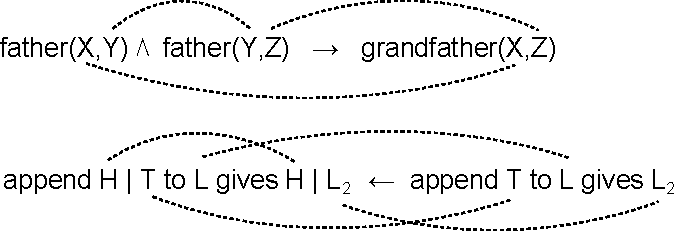
\includegraphics[scale=0.8]{connections-logic-variables.pdf}
\caption{\textcolor{grey}{Linkage of variables in predicate logic: the grandfather rule and the recursive definition of APPEND in PROLOG.}}
\label{fig:ontology-relations-relations}
\end{figure}

\concept{Combinatory logic} is an attempt to eliminate all uses of variable binding in logic;  \concept{Relation algebra} is a restriction of combinatory logic to relational operations.  Genifer3 uses a simplified form of relation algebra.

The bottleneck of AI is in the \concept{learning algorithm}, which will be addressed below.

\section{Logic}

A \concept{formula} in Genifer3 is simply a concatenation of atomic \concept{concepts}:\\
\tab $c_1 \cdot c_2 \cdot ... \cdot c_n$.\\
For example:  \formula{john $\cdot$ loves $\cdot$ mary}.

Since there are no variables in Genifer, \textit{generalization} is achieved via the \concept{subsumption} relation $\subseteq$, for example:\\
\tab \formula{cats $\subseteq$ animals}.\\
This allows to deduce, for example, from \formula{humans are mortal} to \formula{socrates is mortal}.

Logic formulas can be \concept{facts} or \concept{rules};  The difference is that rules are of the form:\\
\tab \formula{pre-condition $\rightarrow$ post-condition}.

As an example consider how one can deduce the new fact:\\
\tab \formula{john $\cdot$ grandfather = paul} \tab (john's grandfather is paul)\\
from the given facts:\\
\tab \formula{john $\cdot$ father = pete}\\
\tab \formula{pete $\cdot$ father = paul}.

This may be achieved via the rule $father \circ father = grandfather$, and the substitution of terms by their equals, but I'm not sure if the substitution operation should or could be reduced to some other logic primitives.

\section{Actions}

We have to pay the price of eliminating logic variables;  One way to do that is via the use of ``memory registers''.

Recall that a Turing machine consists of a tape memory and a set of finite states:
\begin{figure}[H]
\centering
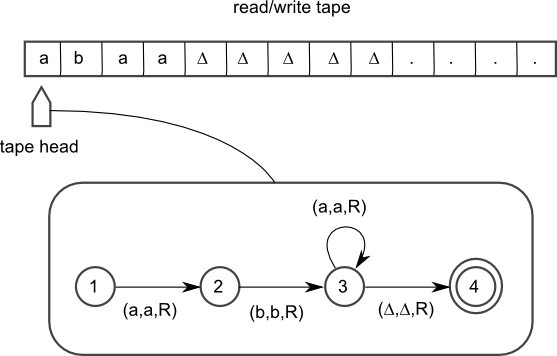
\includegraphics[scale=0.75]{Turing-machine.png}
\caption{\textcolor{grey}{Turing machine that accepts aba*.}}
\label{fig:ontology-relations-relations}
\end{figure}

A logic without variables may be too weak (in the sense that it is no longer Turing-universal).  If we equip the logic with a memory tape (or registers), it would naturally become Turing-universal again.

More concretely, consider this classical logic formula:\\
\tab \formula{raining $\rightarrow$ grass is wet}\\
and we can introduce a new kind of fomulas containing \concept{actions}:\\
\tab \formula{if register A is '0' $\rightarrow$ write '1' into register B}.\\
We can even use data structures such as linked lists and trees instead of simple registeres.  In Genifer 3.0 I am using lists.

\begin{comment}
我们有了动作 但不知道怎样指向\textbf{对象}。 其中一个可能的办法是 用 label 标签上次的答案;  或者作用於所有答案(但这是不自然的?) 

这引申到注意力的问题。  或者 Genifer 永远只是 focus 在注意力的前沿?

还有个问题就是:答案并不一定是唯一的。 所以需要一个方法去把 KB 的答案 掟回到 register 里。  

但那又引申到 working memory 和 KB 的区别。  或者 attention 只是 derivation 的 time-decaying trace?  换句话说,那些可能的答案只有很少几个。  我们应该可以利用某些特徵提取他们。

最简单可能就是 -1 和「没有」的分别。  如何区别「有」和「没有」呢?  可以指定答案的 class,例如「广东话字词」。
\end{comment}

\section{Learning}

The goal of learning is to discover a bunch of logic formulas to \textit{explain} the world.  To explain means to \textit{deduce}.

Learning is achieved through \concept{induction}, that is, to induce \concept{rules} from \concept{facts}.  

In logical notation:\\
\tab $KB \cup H \models E$\\
where KB is the \concept{knowledge base} or background knowledge, H is the new \concept{hypothesis} (to be learned), E is the set of examples or new experience that needs to be explained, and $\models$ denotes \concept{entailment}.

Inductive learning is a search inside the possible space of logic formulas; This search space is huge and our search would be much faster if the space is a lattice, ie, endowed with a \concept{general-to-specific order}. In logic, such an order may be given by:
\begin{enumerate}
\item one concept being more \concept{general} than another concept, for example:\\
\tab \formula{animals $\supseteq$ dogs}
\item adding \concept{conjunctions}, for example:\\
\tab \formula{wear-glasses $\wedge$ has-long-hair}
\end{enumerate}

In Genifer 4 I attempt to switch the setting to continuous space and apply gradient descent, but I am still facing a few unsolved obstacles.  Genifer 3 does not need continuous space, the gradient is no use, so we could simply ``fuck it'' (use a genetic algorithm), which is much easier to do.  Easy does not necessarily mean inferior;  For example, in machine learning competitions, people find out that the most efficient classifiers are based on the theoretically simple \textbf{decision tree} method, rather than the theoretically complex support vector machines.  Perhaps, genetic algorithm is sufficient? :)

\begin{comment}
压缩的方法必须是 ``semantic distance preserving'',意即: 在语义空间中相似的点被压缩到相邻的逻辑範式。

问题似乎是: 法则的诱导似乎不能单是基於语法。 概念阶层的诱导是基於: Liebniz 和 $a R b$。

Liebniz extensionality:
\begin{eqnarray}
xZ \rightarrow yZ \Leftrightarrow x \supset y \\
Zx \rightarrow Zy \Leftrightarrow x \supset y
\end{eqnarray}

The relation of subsumption is \textit{intrinsic} to the logic.  

\begin{tabular}{|c|c|c|c|}
\hline
\textbf{Notation} & \textbf{Meaning} & \textbf{Example } \\
\hline
$A \supset B$ & concept A is a superset of concept B &
$animals \supset cats$ \\
& &  \english{cats are animals} \\
\hline
$A \ni B$        & concept A contains an element concept B &
$a \circ bird \supset tweety$ \\
& & \english{Tweety is a bird} \\
\hline
$A \rightarrow B$ & proposition A entails proposition B &
$bird \, X \supset can \, fly \, X$ \\
& & \english{If X is a bird X can fly} \\
\hline
\end{tabular}

\begin{figure}
\centering
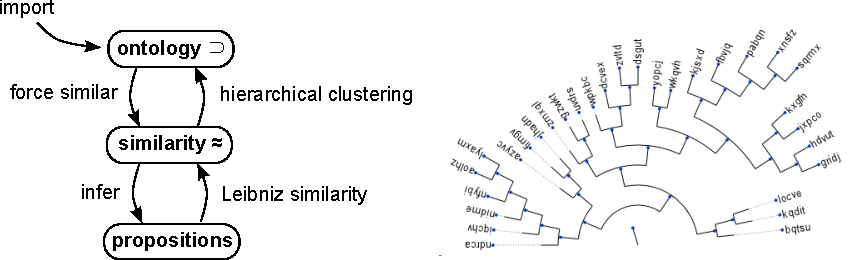
\includegraphics[scale=0.8]{ontology-relations-relations.pdf}
\caption{Left: relations between ontological data.  Right: a random example of dendrogram.}
\label{fig:ontology-relations-relations}
\end{figure}

\section*{Appendix: XXXX}

\end{comment}

\section*{Acknowledgments}

I am heavily indebted to Pei Wang \cite{Wang2006} \cite{Wang2013} and Ben Goertzel \cite{Goertzel2011} for their seminal contributions to AGI.  To Abram Demski and Russell Wallace -- we spent years exploring many ideas in logic.  Also thanks to Matt Mahoney and other participants on the AGI mailing list.  William Taysom, Seh, and Joseph Cheung helped implement the code.

\bibliographystyle{plain} % or number or aaai ...
\bibliography{AGI-book}

\onecolumn

% Bigger figures

\end{document}
